\chapter{Численные результаты}
\section{Описание и подготовка данных}
\indent В работе были использованы данные с 24 каналами и частотой дискретизации 250 Гц для классификации воображаемых движений. Каналы измеряли активность определенных участков коры головного мозга, когда испытуемого просили думать об одном из трех действий: воображаемое движение левой рукой,  воображаемое движение правой рукой и состояние покоя. Соответсвенно, в данных имеется 3 класса состояний. Данные изначально уже были разделены на тестовую и тренировочную выборки: для тестовой выборки испытуемого просили еще раз пройти задание эксперимента.
 
В таблице \ref{tbl:train_data} показаны первые строки имеющихся данных. Все поля содержат в себе некоторые вещественные числа, как правило либо отрицательные, либо положительные. Поле classification принимает одно из значений состояния:  0, 1 или 2.

\begin{table}[h!]
\caption{Тренировочная (исходная) выборка.} \label{tbl:train_data} 
 \begin{center}
  \begin{tabular}{|c|c|c|c|c|c|c|c|}
	\hline  & field1 & field2  & field3 & \ldots & field23 & field24 & classification \\ 
	\hline 0 & -1698.27 & -2227.09 &-3371.32 & \ldots & -7473.05 & -0.01  & 1 \\ 
	\hline 1 & -3369.87 & -4316.49 & -6588.67 & \ldots & -14602.89 & -0.02 & 1  \\
	\hline 2 & -2811.26 & -3658.00 & -5531.58 & \ldots & -12280.18 & -0.017 & 1 \\
%	\hline 3 & -3179.64 & -4083.63 & -6209.13 & \ldots & -13778.39 & -0.019 & 1   \\
%	\hline 4 & -2902.00 & -3765.82 & -5697.67 & \ldots & -12651.33 & -0.017 & 1 \\
	\hline  \vdots & \vdots & \vdots  & \vdots & $\ddots$ & \vdots & \vdots & \vdots \\ 
	\hline 
  \end{tabular} 
 \end{center}
\end{table}

Всего имеет 100717 наблюдений в тренировочной выборке, 100603 --- в тестовой. Для снижения размерности выборок была выполнена передискретизация данных с частотой в 5 раз реже. 

Нужно заметить, что данные в тренировочной и в тестовой сильно отличаются друг от друга. Например, на рис. \ref{img:field4_plots} и \ref{img:field19_plots} изображены сравнительные графики и гистограммы значений полей field и field  в тренировочной и тестовой выборках. Поэтому, перед применением алгоритмов классификации требуется нормализация данных. К тому же, из данных в тренировочной выборке убирались выбросы (для построения стандартных классификаторов).

\begin{figure}[h!]
 \begin{center}
 \begin{minipage}{0.49\linewidth}
    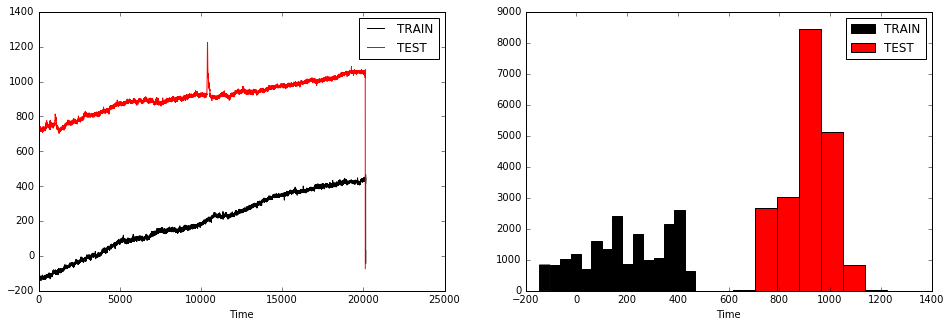
\includegraphics[width = \textwidth]{field4_plots.png}
   \caption{Значения field 4 в тренировочной и тестовой выборках} \label{img:field4_plots}    
  \end{minipage}  
   \hfill
  \begin{minipage}[h]{0.49\linewidth}
      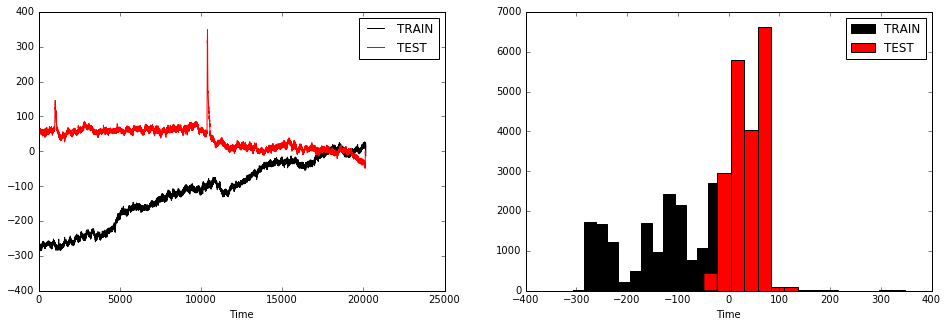
\includegraphics[width = \textwidth]{field19_plots.png}
    \caption{Значения field 19 в тренировочной и тестовой выборках} \label{img:field19_plots}    
  \end{minipage}  
 \end{center}
\end{figure}

\section{Стандартные методы} 
В качестве стандартных методов классификации были использованы линейный дискриминантный анализ (LDA), логистическая регрессия (LogRegression), метод градиентного бустинга (библиотека XGBoost) и Linear SVC (Support Vector Classification). Для рассматриваемых методов данные преобразовывались к значениям от 0 до 1 следующим образом: для вектора $x=\{x_1,~x_2,~\ldots,~x_n\}$ преобразованным вектором назовем $x'=\{x'_1,~x'_2,~\ldots,~x'_n\}$, где $$x'_i = \frac{x_i - \min\{x\}}{\max\{x\} - min\{x\}}$$.
Затем, на вход классификаторам подавались первые три главные компоненты, полученные методом аппроксимации данных principal component analysis (PCA).

Наилучший результат с помощью этих методов удалось получить, используя LDA и логистическую регрессию.

Численное сравнение результатов методов описано в разделе \ref{compute_part:method_compare}.

\section{Классификация с помощью моделей временной иерархической памяти}
С помощью алгоритмов пакета nupic, реализованного на языке Python (2.7), были построены две модели HTM: 
\begin{enumerate}
\item NontemporalClassification;
\item Модель на основе комбинирования MultiStep моделей.
\end{enumerate}
Остановимся на каждой из них подробнее.

\subsection{Модель NontemporalClassification}
Метка Nontemporal в названии модели предполагает, что при такой классификации обученная сеть не запоминает последовательности в данных, а классифицирует каждое наблюдение отдельно. Это свойство делает метод похожим на стандартные методы классификации.

\subsection{Ансамбль MultiStep моделей}
Одним из главных аспектов HTM является работа с непрерывными временными данными. Она основывается на способности Temporal Pooler выучивать временные шаблоны в данных. Поэтому рассмотрим следующую модель:
\begin{itemize}
\item Разделяем тренировучную выборку на имеющиеся классы.
\item Обучаем модель для каждого класса. Для этого внутри классов для каждого из признаков <<field i>> обучается модель предсказания будущих значения; модель строится не только по предыдущим значениям фиксированного признака, но по всех значениям признаков на предыдущих временных отсчетах.
\item Подаем данные из тестовой выборки в каждую из моделей класса (в нашем случае их три).
\item Вычисляем ошибки в предсказаниях на тестовой выборке. 
\item Присваиваем наблюдению тот класс, на котором была достигнута минимальная из посчитанных на предыдущем шаге ошибок.
\end{itemize} 

Проблема модели заключается в больших временных затратах на обучение: имея 3 класса и 24 признака, нужно обучить 72 модели. Одним из вариантов решения является разделение всех признаков на группы коррелирующих между собой и выбор из каждой группы одного представителя, наиболее сильно влияющего на целевую переменную с метками класса.

\section{Сравнение методов}\label{compute_part:method_compare}
В таблице \ref{tbl:results_compare} представлены результаты, полученные с помощью рассматриваемых методов. В качестве мер ошибки использованы мера точности (Accuracy) и F-measure. По результатам видно, что на тестовой выборке ошибка предсказания для модели NontemporalClasification временной иерархической памяти пренебрежимо мала, и точность предсказания значительно превосходит точность стандартных методов классификации для анализировавшихся данных.
 
\begin{table}[h!]
\caption{Сравнение методов классификации.} \label{tbl:results_compare} 
 \begin{center}
  \begin{tabular}{|c|c|c|c|}
	\hline  & Регуляризация & Accuracy & F-measure \\ 
	\hline LDA & $\lambda = 0.2$ & 0.87 & 0.868 \\ 
	\hline Linear SVC (C = 1.0)  & --- & 0.756 & 0.747  \\
	\hline LogRegression  & ---  & 0.877 & 0.88 \\
	\hline XGBoost  &  $\lambda = 0.75$   & 0.787 & 0.79 \\
	\hline NontemporalClassification & --- & 0.999 & 0.999 \\
	\hline 
  \end{tabular} 
 \end{center}
\end{table}
